\chapter{Project overview}
\addcontentsline{toc}{section}{Introduction}


\section*{Introduction}
In this first chapter, we give an overview of the project i'm working on. First, i'll introduce the hosting company that proposed this topic and is hosting it. Next, we describe the project, addressing the problematic and the various objectives to be achieved. We criticize the existing applications and conclude by describing the proposed solution and the methodology adopted.


\section{Hosting company presentation}
AppAxis Innovation is a hosting company that collaborates with developers to create new applications that solve social problems. The company is an expert in mobile development, AI, and web development. AppAxis Innovations offers its support to the pursuit of purposes, which serves as a source of new ideas. It is creativity that finds technical solutions for social needs.
\begin{figure}[H] 
            \centering
            
\includegraphics[scale=0.3]{logos/Full Logo Horizontal Stacked Black PNG.png}
            \caption{AppAxis innovations Logo} 
            \label{fig:Appaxis Logo}
\end{figure}

\section{General context of the project}
This internship is part of an end-of-studies project leading to the national diploma in software engineering at ESPRIT. It is being carried out at Appaxis Innovations, 
a company specializing in developing mobile, web, and AI solutions. The project involves designing and developing a mobile networking application to make life easier for students.

\section{Problematic}
Imagine you're a student in Tunisia. At this stage, you're very excited about enjoying university life, but the harsh reality is that many students feel lonely and disconnected from most things around them. Students may find it difficult to make social connections on campus, as they only have one or two ways to meet and study together or make new friends. This can make their academic activities seem dull and unenjoyable. Transportation problems only make the situation worse and even more annoying. Public transport is often unreliable and may be very expensive, preventing them from commuting and participating in off-campus activities. As a result, most students lose the opportunity to immerse themselves in their interests, bond with their peers, and have a bright academic life, which can lead to :

\begin{itemize}

    \item depression and mental health problems among students.
    \item low self-esteem and poor communication skills .
    \item Poor grades due to lack of concentration and resources.
\end{itemize}

In Tunisia nowadays, the range of students struggling with mental health issues is pretty large, with depression, loneliness, sleeplessness, anxiety, and stress are among the most common problems they face.
\cite{depression_among_tunisian_students}


\section{Study of the existing solutions}

With this understanding, I will share the current situation before presenting possible solutions. Communication and mobility are experienced as problems by students at Tunisian universities. While previous efforts like participating in events or being in the club have been widely used, they cannot be reasonably be compared to the personal atmosphere of unpopular or freshmen students. Alongside trendy under-the-radar apps like Tinder and Bumble, while offering entertainment, their sole purpose is mainly on romantic relations, saving no place for platonic friendships or study groups.
\\
\begin{figure}[H] 
            \centering
            
\includegraphics[scale=0.5]{bumblextinder.png}
            \caption{The most famous meeting apps used in Tunisia: bumble and tinder} 
            \label{fig: meeting appslogos}
\end{figure}
The benefits of using dating apps :

\begin{itemize}
    \item Very popular
    \item Simple user experience
\end{itemize}
but when it comes to drawbacks, dating apps :

\begin{itemize}
    \item Has been considered inappropriate and they are therefore not much of a favorite with the users.
    \item It is filled with fake profiles and could open the user up to con artists and people who might make the user uncomfortable.
    \item Only deals with romantic relationships. This may not be in line with the Tunisian students who are looking for purely platonic relationships or just group studies.
    \item Many complaints of users experiencing acts of harassment that make them or other users feel insecure.
\end{itemize}

Such applications can embarrass students especially the shy and less experienced ones, because these have nothing to do with the interaction of the dating apps.
\\
\\
Let's not forget about the tried and tested methods such as enrollment for competitions or joining clubs that have been here for decades. The formation of friendships among them is dependent on the mere ongoing conversation on the campus.
\begin{figure}[H] 
            \centering
            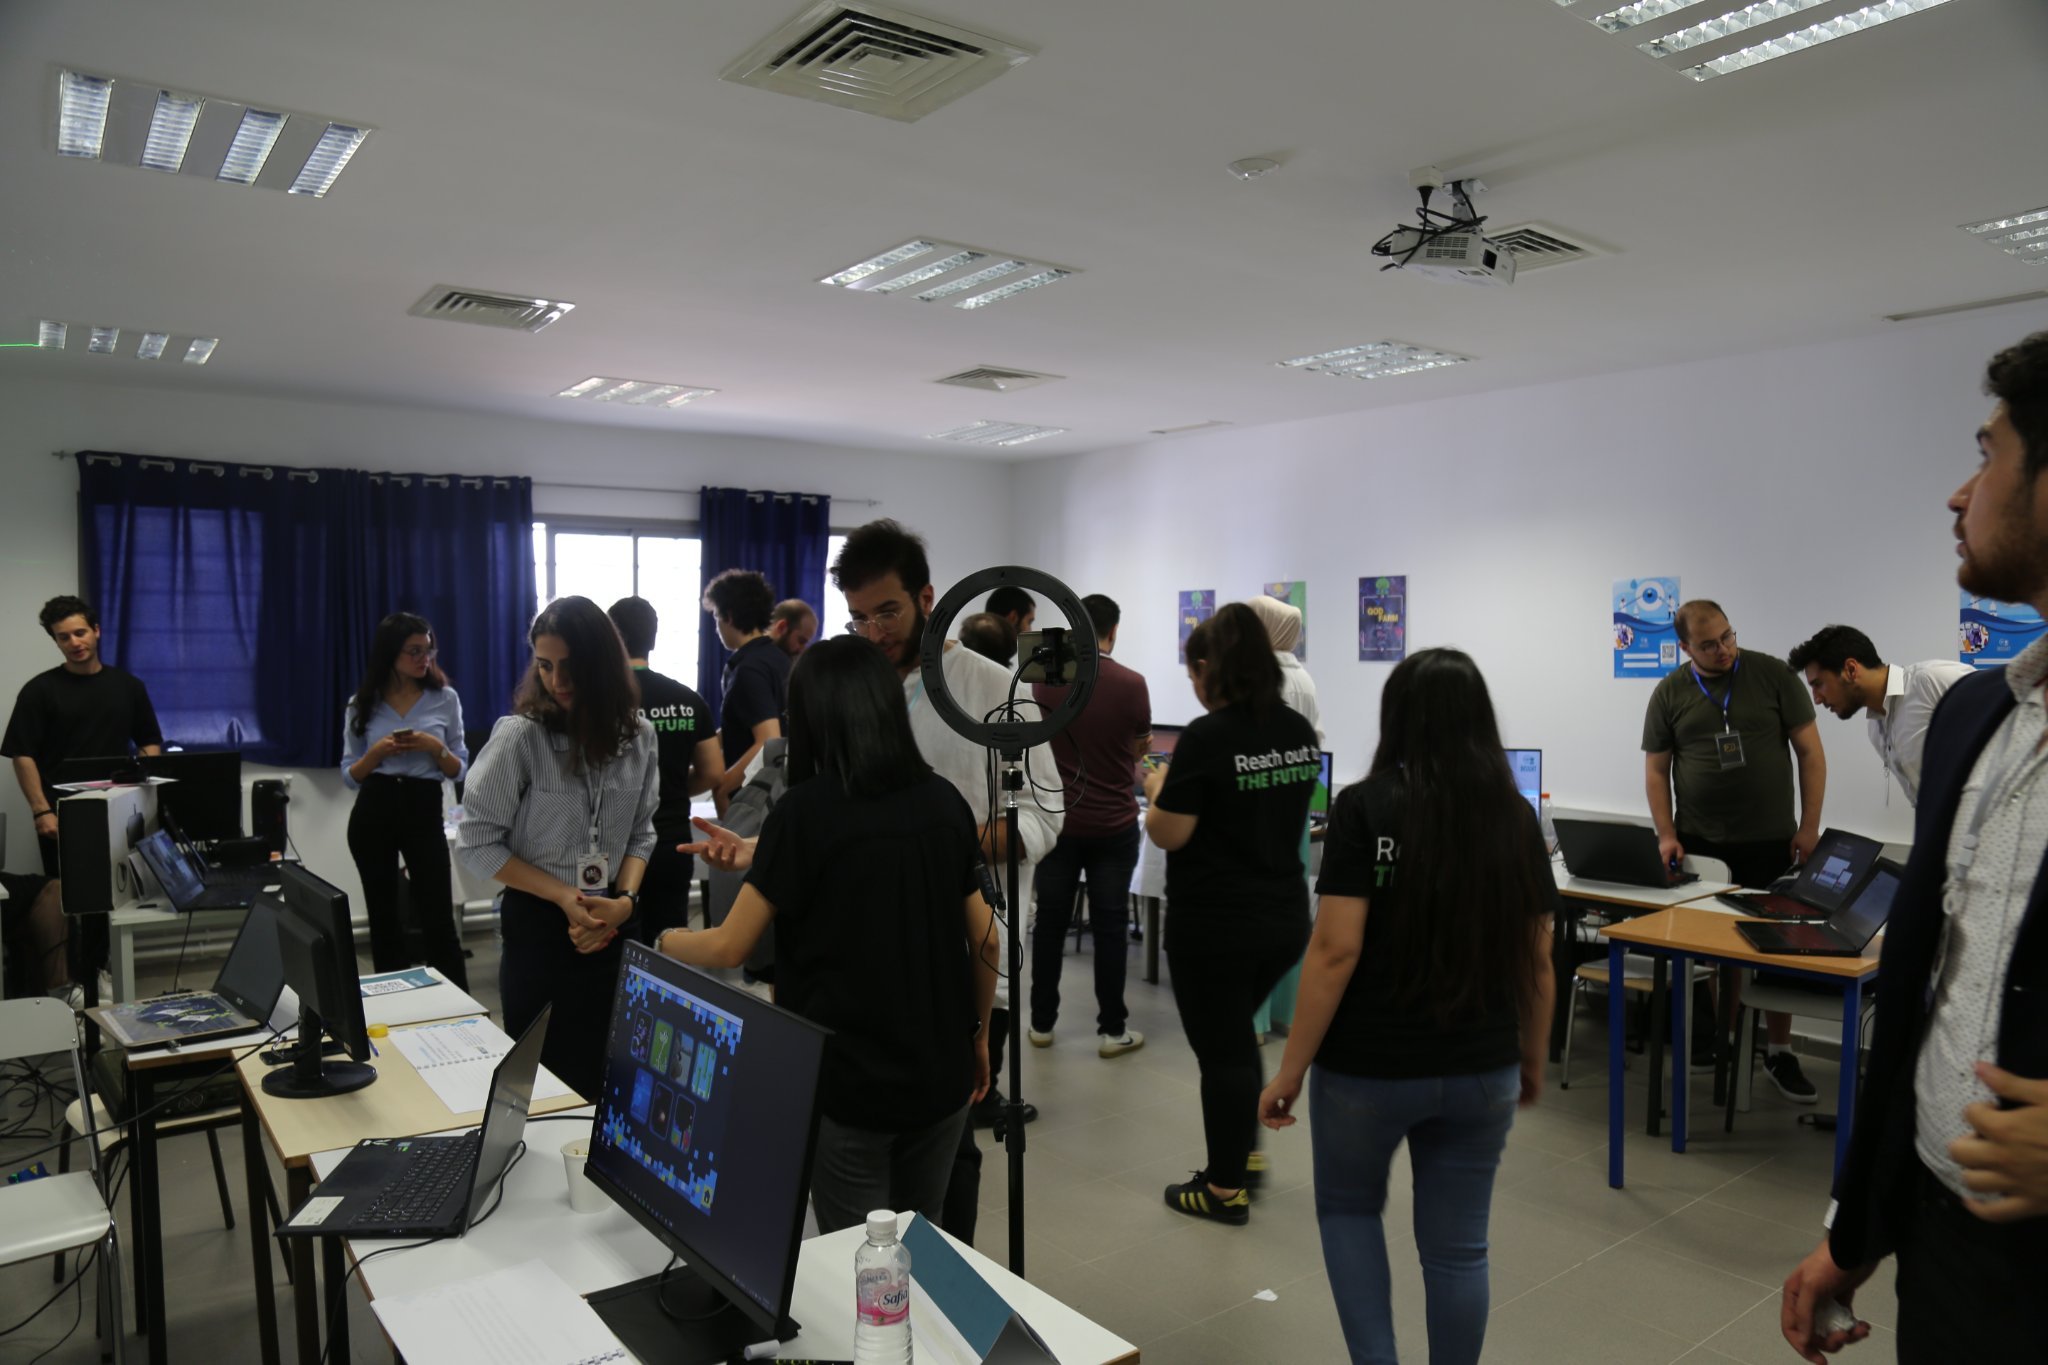
\includegraphics[scale=0.15]{event.jpg}
            \caption{One of the most famous events in esprit: bal des projets} 
            \label{fig: Student events exemple}
\end{figure}
Sometimes, it is very difficult for reserved and shy students to walk into a room full of unknown individuals. In addition, this approach is not guarantee of friendships of lasting significance as opposed to the case in a cultural setting like Tunisia where the norms may differ.
Regarding transport, we find that a majority of the bus service users or the demand that come from Tunisia are the school and university students, where in 2019 they represented 53\% of the entire population and are constantly on the rise. \cite{Share_of_students_in_total_bus_passengers}
\begin{figure}[H] 
            \centering
            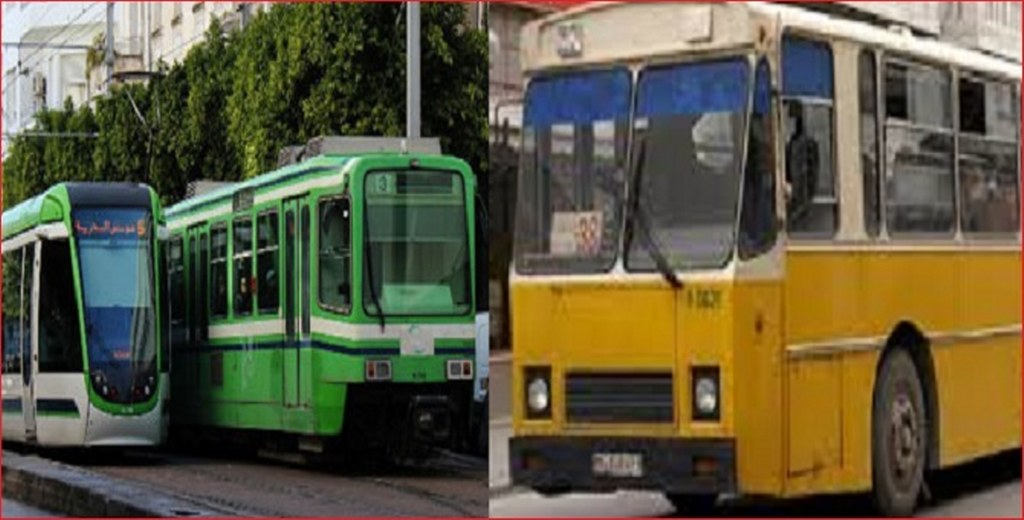
\includegraphics[scale=0.3]{bus-metro-tunis.jpeg}
            \caption{example of public means of transportation: bus and metro} 
            \label{fig: example of means of transportation}
\end{figure}
Even though, using public transport to get to university may be convenient and costs mere money, it has certain disadvantages:
\begin{itemize}
    \item lack of safety.
    \item very tiring
    \item time-consuming
    \item lack of comfort
\end{itemize}
To avoid that, some students use taxis, which offers comfort and fast service, but also has its drawbacks: 
\begin{itemize}
    \item taxis can be very expensive if they are a daily means of transport.
    \item taxis can be hard to find in some areas
    \item sometimes unavailable
\end{itemize}
\begin{figure}[H] 
            \centering
            \includegraphics[scale=0.2]{Taxis_in_Tunesien.jpg}
            \caption{example of means of transportation: Taxis} 
            \label{fig: example of means of transportation 2}
\end{figure}
Students in a rush usually opt for private cabs provided by apps, like Bolt and inDrive. All the same, such cabs have disadvantages and one of the biggest reasons students do not use them often is because most of them are not cost-effective or even affordable to some people.
\begin{figure}[H] 
            \centering
            
\includegraphics[scale=0.5]{apps_logo.png}
            \caption{example of Transportation applications: Bolt and inDrive} 
            \label{fig: example of Transportation apps}
\end{figure}

So, since not all existing solutions are suitable for students, how can we meet their needs?

\section{Proposed solution}
Though the above solutions may work for some, they have their own problems and limitations and cannot work for students overall, because students are very sensitive target. \\
That’s why uni-world thought of satisfying students’ needs by taking the drawbacks of all existing solutions and correcting them to give us the best solution for students. \\

Uni-world is divided into two modes: uni-match and uni-carpool.
\begin{itemize}
\item uni-match is a space for students to meet and make new friends in a safe, easy, and fun way, solving the problems of the usual dating apps.
\item uni-carpool is an environment for students looking for transportation and for those who want to earn money. uni-carpool enables students to find or create carpooling opportunities.
\end{itemize}


\section{Methodology process}

When designing an application as complex as Uni-World, which is best built to respond to users daily needs and frequently change, the project’s management structure must be equally fluid and adaptive. Therefore, this project opted for Agile methodology because it is flexible, and involves constant increment and enhancement processes. 
\subsection{Agile Methodology}
When it comes to projects, agile methodologies are perfect, and they are implemented when the requirements are not clearly outlined, or when the customers expect changes on the application. The basis for our work in the development of “Uni-world” We have decided to choose one of the currently popular methods, namely SCRUM.
Speaking about the methods of project management and taking into account such a great number of available methods, we have decided to use the SCRUM method for the development of the “Uni-World”. \\

\subsection{Chosen Methodology: Scrum}
The Scrum Method is one of the Agile frameworks that divides the developmental process into iterations that are time-bound and commonly known as sprints. The best practice in this development is called Scrum which entails various roles as well as artifacts that act as crucial events. \\ \\
Key Components of Scrum: 
\begin{itemize}
    \item Roles:
    \begin{itemize}
    \item Product Owner: Acts as a representative of the stakeholders and is charged with the responsibility of outlining and prioritizing of the product backlog.
    \item Scrum Master: Coaches in Scrum, enforces the use of Scrum practices, and dissolves impediments.
    \item Development Team: A team which is composed of members from different divisions and who is accountable for the delivery of the item of work for the product increment.
\end{itemize}
    \item Events:
    \begin{itemize}
    \item Sprint Planning: A process of planning what has to be achieved in the current sprint and which items from the product backlog should be developed.
    \item Daily Standup: Specifically, Scrum refers to a 15-minute daily communication, where the team reports to one another regarding the work completed, work to be done and possible obstacles.
    \item Sprint Review: A face-to-face or video conference near the end of the sprint during which the stakeholders are presented with the work that has been done and their input is taken.
\end{itemize}   
\item Artifacts:
\begin{itemize}
    \item Product Backlog: This denotes an arrangement of features, enhancements, and fixes essential for the product. Sprint Backlog: It is a list of tasks to be taken up during the sprint which is culled out from the product backlog.
    \item Increment: This is a precise or concrete product obtained at the end of every sprint.
\end{itemize}
\end{itemize}

\begin{figure}[H] 
            \centering
            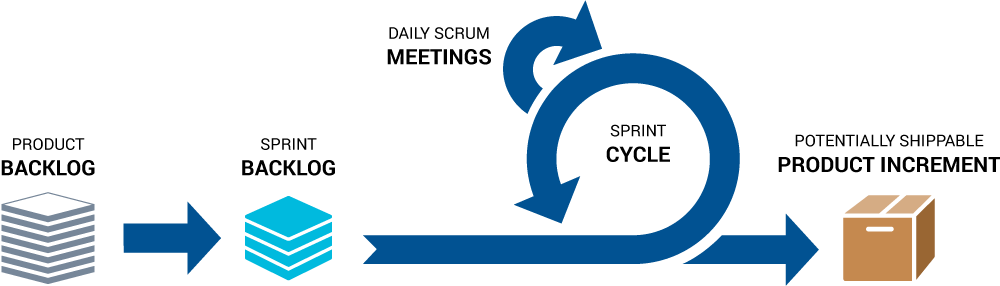
\includegraphics[scale=0.45]{agile.png}
            \caption{Agile Software Development Methodology SCRUM} 
            \label{fig: Agile Software Development Methodology SCRUM}
\end{figure}
\subsection{Why SCRUM ?}
We chose SCRUM because of its three-pillar foundation:We chose SCRUM because of its three-pillar foundation:
\begin{itemize}
    \item Inspection: again and again, Scrum tries to make it compulsory to assess differently. created to identify if there was any shift in their design towards the negative direction. These inspections should not be conducted in such a manner that it results in a negative impact on the health of citizens, the economy, or the environment.
    be carried out too frequently, or by a poorly-trained inspector: this would retard the project progress.
    \item Transparency: Communication is at the core of scrum since all the development activities are centered on a common language.
    \item Adaptation: This again means that when a deviation is noted during inspection the process must be halted.
\end{itemize}
\subsection{Scrum team structure}
As we have opted for a Scrum method, the role distribution will be as 
follows in the Table below:
\begin{table}[h]
    \centering
    \begin{tabular}{|p{3cm}|p{4cm}|p{8cm}|}
        \hline
        Role & Actor & Mission\\
        \hline
        Product Owner & Mouheb eddine saadaoui & Responsible for updating and managing the product backlog. \\
        \hline
        Scrum Master & Ahmed hchaichi & Responsible for establishing Scrum and team efficiency. \\
        \hline
        Scrum Team & Bairem khedhri & Responsible for the development of the product \\
        \hline
    \end{tabular}
    \caption{Text description of the carpooling offer management use case}
    \label{Tab: Text description of the carpooling offer management use case}
\end{table}


\section*{Conclusion}
In this first chapter, we discussed the project as a whole. First, we took a look at the general context of the project to understand the project in a nutshell, then moved on to the presentation of the hosting company. Following this, we saw the problem and how the students were struggling, we had a look at the existing solutions and critiqued them to see their shortcomings and how to remedy them, and finally, we presented the methodology we are adopting in the project. In the next chapter, we'll look at the functional and technical aspects of the application.

 
  